\section{Experimental Protocols and Results}
\label{app:d}\label{app:experiments}

This appendix specifies the experiments in Section~\ref{sec:experiments}:
finite-cell identification and estimation, historical applicant assessment,
controlled masking, and targeted revelation. All results use saved outputs;
Appendix~\ref{app:implementation-inventory} identifies the accompanying provenance.

\subsection{Evaluation targets, interval construction, and aggregation}
\label{app:evaluation-targets}

Write $\beta=1-\alpha$, $\rho^L=\underline\rho_{\alpha,\Gamma}$,
$\rho^U=\overline\rho_{\alpha,\Gamma}$, and $I_\Gamma=\rho^U-\rho^L$.
Endpoints minimize their respective threshold objectives. Finite-support minima
are found exactly at $0$, $1$, and all label-specific loss breakpoints, including
when estimated hinge coefficients are signed. Sampling and lending studies use
Brier loss $(f-y)^2$; population sweeps and the synthetic frontier use absolute loss.

\begin{center}
\small\setlength{\tabcolsep}{3pt}
\begin{tabularx}{\textwidth}{@{}>{\raggedright\arraybackslash}p{.19\textwidth}>{\raggedright\arraybackslash}X>{\raggedright\arraybackslash}X>{\raggedright\arraybackslash}p{.18\textwidth}@{}}
\toprule
Study & Target & Metric & \shortstack[l]{Replications/\\aggregation}\\
\midrule
Finite-cell sampling & Sharp population interval; its endpoints & Oracle whole-interval containment; learned-endpoint RMSE & 60 worlds $\times$ 80 samples per $n$; means/RMSE\\
Historical applicants & Applicant-level regression-extension sensitivity interval & Estimated endpoints and strict comparisons & One cohort; five-fold cross-fitting\\
Controlled masking & Full-outcome CVaR of each fitted predictor & Reference coverage; comparison errors and unresolved decisions & 20 masks; counts and mean widths\\
Fixed revelation & Fixed-threshold retained gap $W_{f,\eta}$ & Remaining gap; cost to target & 120 synthetic worlds or 20 masks; within-run normalization, then medians/IQR\\
Sequential audits & Estimated optimized retained width; held-out predictive loss & Width, mean Brier loss, CVaR; paired TIV--random differences & 20 masks; medians and descriptive IQR\\
\bottomrule
\end{tabularx}
\end{center}

For fixed $f,\eta$, the revelation target is
$W_{f,\eta}(\lambda)=\E[(1-\lambda)\tau_{f,\eta}]$, where
$\tau_{f,\eta}=(1-\pi)s_\Gamma|d_{f,\eta}|/\beta$.
It differs from the optimized width, whose endpoints are minimized separately
(Appendix~\ref{app:optimized-width}). Oracle containment, masking-reference
coverage, and sequential plug-in precision have different calibration premises.
Fixed-audit reductions normalize within each run before aggregation; sequential
widths aggregate the recorded widths. Ratios of separately aggregated values
need not equal aggregated relative reductions.

\subsection{Finite-cell identification and learned-endpoint accuracy}
\label{app:finite-sample-experiments}

\paragraph{Generator and estimators.}
Each of 60 simulated populations has covariate support $\mathcal X_0$ consisting of 30
cells, with Dirichlet$(1,\ldots,1)$ masses, independent $\pi\sim U[.2,.95]$ and $p_1\sim
U[.05,.95]$, and $p_0\mid p_1\sim U[q_-(p_1),q_+(p_1)]$ at $\Gamma=2$.

Fix $f=\operatorname{clip}_{[0,1]}(p_1+N(0,.15^2))$ within each world,
use Brier loss and $\alpha=.75$, and compute exact endpoints and generating-law
CVaR on $T_f=\{0,1\}\cup\{f(x)^2,(1-f(x))^2:x\in\mathcal X_0\}$.
For each $n\in\{1000,3000,10000,30000,100000\}$, draw 80 samples per world
(4,800 replications). The oracle uses known $p_1$ and the bounded score of
Appendix~\ref{app:oracle-calibration}; its endpoints are expanded by
\[
r_{\rm or}=\frac1\beta\sqrt{\frac{\log(4|T_f|/\delta)}{2n}},\qquad \delta=.05,
\]
then clipped to $[0,1]$. Proposition~\ref{prop:b:oracle-calibration} gives
whole-interval containment with probability at least $.95$ for this fixed predictor.
Saved generating-law CVaR coverage also equals one at every reported sample size.

On the same records, randomly assign each observation to one of two folds. In a given training cell, let $N_{11}$ count records with $(S,Y)=(1,1)$, let $N_{10}$ count records with $(S,Y)=(1,0)$, and let $N$ be the total number of training records in that cell. Estimate
\[
\widehat p_1=\frac{N_{11}+1/2}{N_{11}+N_{10}+1},
\qquad
\widehat\pi=\frac{N_{11}+N_{10}}{N},
\]
clipped to $[.01,.99]$ and $[.1,1]$, respectively; an empty training cell receives propensity $1/2$. Evaluate the locally robust score using the other fold's fits. The resulting RMSEs measure endpoint accuracy. Learned-nuisance coverage requires a separate calibration argument.

\begin{table}[!htbp]
\centering\small
\setlength{\tabcolsep}{4pt}
\begin{tabular}{rcccccc}
\toprule
$n$ & Sharp width & Radius & Outer width & Coverage & RMSE upper & RMSE lower\\
\midrule
1{,}000 & .0949 & .260 & .614 & 1.000 & .0361 & .0425\\
3{,}000 & .0949 & .150 & .395 & 1.000 & .0171 & .0160\\
10{,}000 & .0949 & .082 & .259 & 1.000 & .0087 & .0076\\
30{,}000 & .0949 & .047 & .190 & 1.000 & .0049 & .0043\\
100{,}000 & .0949 & .026 & .147 & 1.000 & .0027 & .0023\\
\bottomrule
\end{tabular}
\caption{Repeated-sampling decomposition over 4,800 replications per sample size.
Widths and oracle radii are means; coverage is the proportion of oracle outer
intervals containing both exact endpoints. RMSE uses two-fold learned-nuisance estimates
on those same sampled records.}
\label{tab:finite-sample}
\end{table}

\paragraph{Observed-tail scaling.}
For the $d=16$ tail-cell construction of Appendix~\ref{app:learning-lower-bound}, use 240 replications at each of 54 settings:
$n\in\{600,900,1400,2200,3500,5500\}$,
$\beta\in\{.10,.15,.25\}$, and $\pi_0\in\{.20,.35,.55\}$.
Set $\gamma=\min\{.20,.16\sqrt{d/(n\beta\pi_0)}\}$ and recover each cell's
sign by majority vote among revealed tail labels, assigning ties the positive sign.
The metric is $2\gamma$ times the incorrectly recovered fraction, equal to excess
CVaR for this construction. Its least-squares guide against
$1/\sqrt{n\pi_0\beta}$ has slope $.5030$, intercept $-.0018$, and
$R^2\simeq.998$; this illustration does not establish a general matching upper
bound for Appendix~\ref{app:learning-lower-bound}.

\paragraph{Population sweeps.}
The five-region absolute-loss design has region masses $\mu_j=P(X=j)$ and full-data outcome probabilities $p_{\mathrm{full},j}=P(Y=1\mid X=j)$, for $j=1,\ldots,5$. It fixes
\[
\begin{aligned}
\mu&=(.45,.15,.15,.10,.15),&p_{\rm full}&=(.04,.75,.10,.40,.50),\\
s_1&=(.80,.03,.80,.80,.80),&s_0&=(.80,.60,.80,.80,.80),\\
f&=(.05,.25,.10,.40,.50),&&s_y=P(S=1\mid X,Y=y).
\end{aligned}
\]
Exact finite-support optimization evaluates 60 tail levels on $[.55,.95]$ at
$\Gamma=50$, and 60 common historical observation probabilities on $[.05,1]$ at
$\alpha=.85,\Gamma=50$, holding the original $p_1$ fixed in the latter sweep.
An archived sweep uses 60 log-spaced $\Gamma\in[1,100]$ at $\alpha=.85$;
values below the generating sensitivity shift do not claim generating-law coverage.

\begin{figure}[!tbp]
\centering
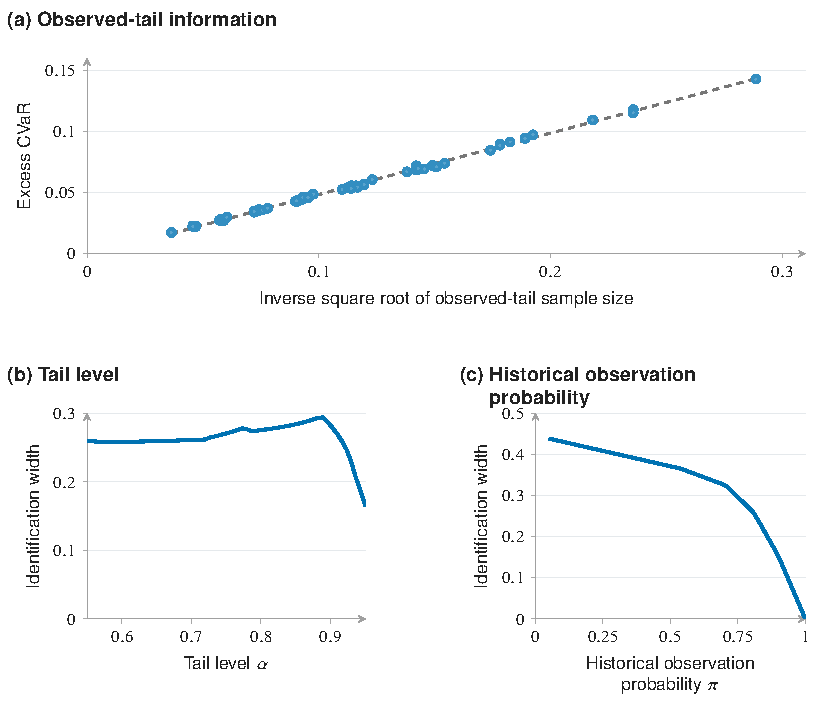
\includegraphics[width=\textwidth]{figures/supp_diagnostics.pdf}
\caption{\textbf{Observation scarcity and sensitivity shape tail-risk precision.} (a) Recorded
simulations of the Appendix~\ref{app:learning-lower-bound} learning construction, with a
least-squares guide against $(n\pi_0\beta)^{-1/2}$. Here $n\pi_0\beta$ is the expected
observed-tail sample count. (b--c) Exact identification widths for the fixed five-region
design as the tail level or historical observation probability varies. Width can vary
nonmonotonically with $\alpha$. Lines join recorded evaluations.}
\label{fig:diagnostics}
\end{figure}

\subsection{Historical LendingClub applicant assessment}
\label{app:historical-lending}

\paragraph{Cohort and shared preprocessing.}
From the public 2007--2018 accepted/rejected files \citep{george2019lendingclub},
retain loans issued and applications rejected in 2012. Mature issued outcomes
are charged-off/default ($Y=1$) or fully paid ($Y=0$), including corresponding
former-credit-policy statuses; exclude non-mature outcomes. The saved cohort has
390,644 applications: 53,367 issued loans (8,644 defaults) and 337,277 rejections.
Repayment under issuance is unobserved for rejected applications.

Features are recorded amount, debt-to-income ratio (DTI), FICO credit-score interval
midpoint or recorded risk score, employment years, state, three-digit ZIP prefix, and normalized purpose; exclude
accepted-only pricing/repayment fields, policy code, and calendar month.
Within each training sample, median-impute numeric fields with missingness
indicators, most-frequent-impute categorical fields, and one-hot encode categories
with minimum frequency 25. Standardize numeric fields for logistic regression.
Preprocessing, logistic regression, and stratified splitting use scikit-learn
\citep{pedregosa2011scikit}.

\paragraph{Eligibility, measurement, and extrapolation.}
\label{app:scope-support}
The 2012 FICO minimum was 660 \citep{lendingclub2012registration}.
Source checks identify 180,903 below-660 applications (46.31\%) and 23,097
missing standardized scores, with no issued loans in either group. All 53,367
issued loans lie among the remaining 186,644 records at or above 660.
This structural restriction does not make FICO eligibility sufficient for joint
covariate support or other underwriting requirements.

Recorded fields also differ \citep{lendingclubdictionary}: rejected applications
record FICO, whereas issued loans use an origination-score interval midpoint,
without common coarsening; issued \texttt{loan\_amnt} can reflect credit-department
reductions, whereas rejected \texttt{Amount Requested} is the requested total.
Issued purpose categories and rejected free-text titles are regex-normalized;
dates refer to funding month and application date, respectively. Thus these are
not identically measured predecision covariates.

In training fold $-k$, fit the issued-outcome regression $\widehat r_{-k}$ using
the boosting settings below, evaluate every held-out record, and specify
\begin{equation}\label{eq:d:historical-extension}
r_i=\operatorname{clip}_{[.01,.99]}\widehat r_{-k(i)}(X_i),
\qquad q_i\in[q_-(r_i),q_+(r_i)].
\end{equation}
On unsupported recorded covariates, $r_i$ is an extrapolated reference, not an
identified selected-label probability. Objectives use \eqref{eq:robust-score}
with $p=r_i$, clipped fitted propensity, and the selected-observation residual
correction. These residual-adjusted model-based estimates do not satisfy the
population-overlap premise of Theorem~\ref{thm:learning} on the full cohort.

\paragraph{Models, cross-fitting, and optimization.}
Candidates use standard classification objectives: $\ell_2$ logistic regression
($C=1$, L-BFGS, 1000-iteration limit), default-weighted logistic regression
(default class weight 2), and XGBoost \citep{chen2016xgboost} (450 trees,
depth 5, learning rate $.04$, minimum child weight 10, row/column subsampling
$.85$, $\ell_2$ penalty 2, histogram trees, recorded CUDA configuration).
Both nuisance classifiers use the boosting settings with separately fitted
preprocessing and distinct seeds: $p_1$ uses revealed outcomes and $\pi$
predicts $S$ from all training covariates. Shuffled five-fold cross-fitting is
stratified by $S$; clip $\widehat p_1$ to $[.01,.99]$ and $\widehat\pi$ to
$[.02,.98]$. Evaluate Brier loss at $\alpha\in\{.90,.95\}$ and
$\Gamma\in\{1,1.25,1.5,2,3,5,8,12\}$.

The corrected objective can be nonconvex because hinge coefficients can be signed. Enumerate
$0$, $1$, and both label-specific losses, $f(X_i)^2$ and $(1-f(X_i))^2$, at every observed
covariate $X_i$, including records whose actual outcomes are hidden. Deduplicate and sort
increasingly; among exactly equal computed minima, choose the smallest threshold, without
numerical tie tolerance. Clip endpoints to $[0,1]$; if they cross, replace both by their
midpoint. These clipping and crossing conventions are computational operations and do not
supply statistical coverage.

\paragraph{Fold enlargement and diagnostics.}
At each endpoint's selected threshold, compute five fold-specific objectives and divide
their sample standard deviation by $\sqrt5$ to obtain an empirical standard error. Let
$t_{.975,4}$ be the .975 quantile of a Student-$t$ distribution with four degrees of
freedom. Subtract this multiplier times the lower-endpoint standard error from the raw lower
endpoint and add the corresponding upper-endpoint quantity to the raw upper endpoint, before
clipping or crossing repair. Then clip both limits to $[0,1]$ and order them by minimum and
maximum. This empirical diagnostic uses dependent fold-specific quantities because their
training samples overlap; calibrated coverage requires the conditions and radius of
Theorem~\ref{thm:learning}.

Historical propensity AUC is $.9944$ and Brier score $.0201$; raw propensities
are below $.02$ for 75.26\% and above $.98$ for 1.80\% of applicants, and
inverse clipped propensities are at most 50, indicating substantial extrapolation.
Subgroups reuse full-cohort cross-fitted predictions and require at least
$\max\{250,\lfloor.002N\rfloor\}$ applications and 50 issued loans.
At $\Gamma=2,\alpha=.95$, boosting width is $.080$ for DTI above 30\%
(2.7\% issued) and $.032$ for FICO 700--739 (30.3\% issued).

\begin{table}[!htbp]
\centering\small\setlength{\tabcolsep}{3pt}
\begin{tabular}{llcccc}
\toprule
$\alpha$ & Predictor & Accepted-only & $\Gamma=1$ & $\Gamma=2$ & $\Gamma=3$\\
\midrule
.95 & Gradient boosting & .795 & .733 & [.703,.759] & [.682,.773]\\
.95 & Logistic & .801 & .805 & [.770,.831] & [.745,.843]\\
.95 & Default-weighted & .661 & .813 & [.782,.833] & [.757,.841]\\
.95 & Constant $1/2$ & .250 & .250 & [.250,.250] & [.250,.250]\\
.90 & Gradient boosting & .740 & .679 & [.625,.715] & [.575,.732]\\
.90 & Logistic & .741 & .721 & [.669,.760] & [.631,.778]\\
.90 & Default-weighted & .579 & .720 & [.679,.747] & [.646,.759]\\
.90 & Constant $1/2$ & .250 & .250 & [.250,.250] & [.250,.250]\\
\bottomrule
\end{tabular}
\caption{Historical applicants: accepted-only CVaR and model-based applicant-level
sensitivity intervals. Values other than the exact constant reference are estimates.
At $\Gamma=1$ the reference model fixes the hidden probabilities. Default-weighted denotes logistic
regression with default class weight 2.}
\label{tab:lc-parta}
\end{table}

For $f\equiv1/2$, both label-specific Brier losses equal $1/4$. Mean loss and every CVaR
endpoint therefore equal $1/4$, and $d_{f,\eta}=\mathrm{TIV}=0$ for every threshold. This
row provides an exact predictor reference; the acquisition policies compare audits for a
fixed or sequentially refitted boosting predictor.

\paragraph{Off-grid breakdown.}
For an accepted-only preferred $f$ and comparator $g$, set
$G(\Gamma)=\widehat\rho^L_\Gamma(g)-\widehat\rho^U_\Gamma(f)$.
At the first grid value $\Gamma_+$ with $G(\Gamma_+)\leq0$, if its predecessor
$\Gamma_-$ has positive gap, interpolate:
\[
\log\widehat\Gamma_{\rm br}=\log\Gamma_-+
\frac{G(\Gamma_-)}{G(\Gamma_-)-G(\Gamma_+)}
(\log\Gamma_+-\log\Gamma_-).
\]
These values interpolate the recorded grid. Boosting versus logistic gives approximate
breakdown $2.24$ at $\alpha=.95$, with first failed grid value 3, and $1.40$ at
$\alpha=.90$, with first failed value 1.5. Default-weighted versus logistic gives
approximately $1.01$ at $\alpha=.90$, with first failed value 1.25. The other three
accepted-only orderings fail already at $\Gamma=1$. A comparison with no crossing through 12
is recorded as right-censored above the grid.

\begin{figure}[!t]
\centering
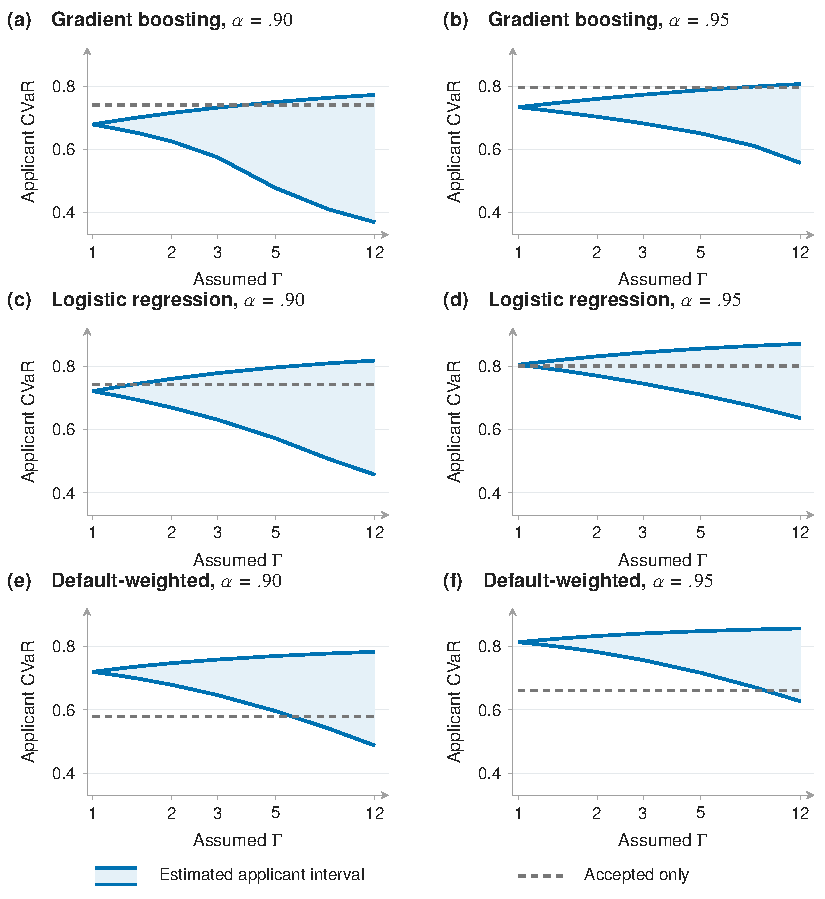
\includegraphics[width=\textwidth]{figures/supp_sensitivity.pdf}
\caption{\textbf{Complete applicant-level sensitivity analysis.}
All three predictors at $\alpha=.90$ and $.95$ over eight recorded sensitivity
levels. Blue boundaries and shading show estimated sensitivity endpoints under the applicant regression extension of Appendix~\ref{app:historical-lending}. Gray dashed lines show accepted-only CVaR. Horizontal
axes are logarithmic and vertical limits are shared. Default-weighted denotes
default-weighted logistic regression.}
\label{fig:full-sensitivity}
\end{figure}

\subsection{Controlled masking: empirical coverage and model comparisons}
\label{app:controlled-masking}\label{app:statistical-scope}

For the 53,367 mature issued loans with known outcomes, independently draw 20
masks from
\[
\begin{aligned}
\operatorname{logit}P(S=1\mid X,Y)&=c+g(X)-Y\log3,\\
g(X)&=\operatorname{clip}_{[-3,3]}\bigl\{.65z(\text{score})-.35z(\text{DTI})\\
&\hspace{90pt}+.15z(\log(1+\text{amount}))\bigr\}.
\end{aligned}
\]
Each $z$ standardizes the median-imputed pseudo-population feature. Solve for
expected revealed share $.45$ ($c=-.0423744$). Bayes' rule gives
$\odds(p_0)/\odds(p_1)=3$, hence $\Gamma_0=3$; boundary outcome probabilities
coincide across hidden/revealed groups as in Appendix~\ref{app:compatibility}.
This validates artificial masking of mature issued loans, not outcomes for
historically rejected applicants.

All three predictors share shuffled five-fold splits stratified by imposed $S$; fitting,
clipping, threshold search, and fold enlargement follow
Appendix~\ref{app:historical-lending}. Reference CVaR uses every known outcome with that
predictor's cross-fitted predictions. Table~\ref{tab:lc-partb} counts intervals containing
this full-outcome reference risk. Table~\ref{tab:mask-comparisons} checks strict separation
of plug-in intervals against reference risk orderings. Three unordered predictor pairs per
mask and 20 masks give 60 comparisons at each tail level, or 120 across both levels.

\begin{samepage}
Figure~\ref{fig:detailed-coverage} retains the complete assumed-$\Gamma$ grid; plug-in
coverage is zero at every tested $\Gamma\le2$. Main-figure pooling averages 20 mask-level
means over three predictors, giving 60 equally weighted predictor--mask rows from 20
independent masks. Fold enlargement is an empirical calibration diagnostic; the class-wide
calibrated statement is Theorem~\ref{thm:learning}.
\par\end{samepage}

\begin{table}[!htbp]
\centering\small\setlength{\tabcolsep}{3pt}
\begin{tabular}{llcccc}
\toprule
$\alpha$ & Predictor & Plug-in & Enlarged & Mean width & Enlarged width\\
\midrule
.90 & Gradient boosting & 11/20 & 19/20 & .401 & .434\\
.90 & Logistic & 13/20 & 20/20 & .401 & .434\\
.90 & Default-weighted & 14/20 & 20/20 & .332 & .365\\
.95 & Gradient boosting & 14/20 & 19/20 & .070 & .089\\
.95 & Logistic & 12/20 & 20/20 & .066 & .084\\
.95 & Default-weighted & 14/20 & 20/20 & .110 & .139\\
\bottomrule
\end{tabular}
\caption{Controlled masking at $\Gamma=\Gamma_0=3$. The middle columns count
intervals covering the full pseudo-population reference CVaR over 20 masks;
the last two columns are mean widths. Fold enlargement follows the empirical diagnostic in Appendix~\ref{app:historical-lending}.}
\label{tab:lc-partb}
\end{table}

\begin{table}[!htbp]
\centering\small
\setlength{\tabcolsep}{7pt}
\begin{tabular}{@{}llrrrr@{}}
\toprule
$\Gamma$ & $\alpha$ & Comparisons & Resolved & Incorrect & Unresolved\\
\midrule
3 & .90 & 60 & 0 & 0 & 60\\
3 & .95 & 60 & 37 & 0 & 23\\
1 & Both levels & 120 & 120 & 16 & 0\\
\bottomrule
\end{tabular}
\caption{Model comparisons under controlled masking. Strict separation of plug-in intervals declares
an ordering, whose correctness is checked against known-outcome reference CVaRs. Counts give
resolved pairs, incorrect declared orderings, and unresolved pairs. Each tail level includes
three unordered predictor pairs in each of 20 masks.}
\label{tab:mask-comparisons}
\end{table}

\begin{figure}[!t]
\centering
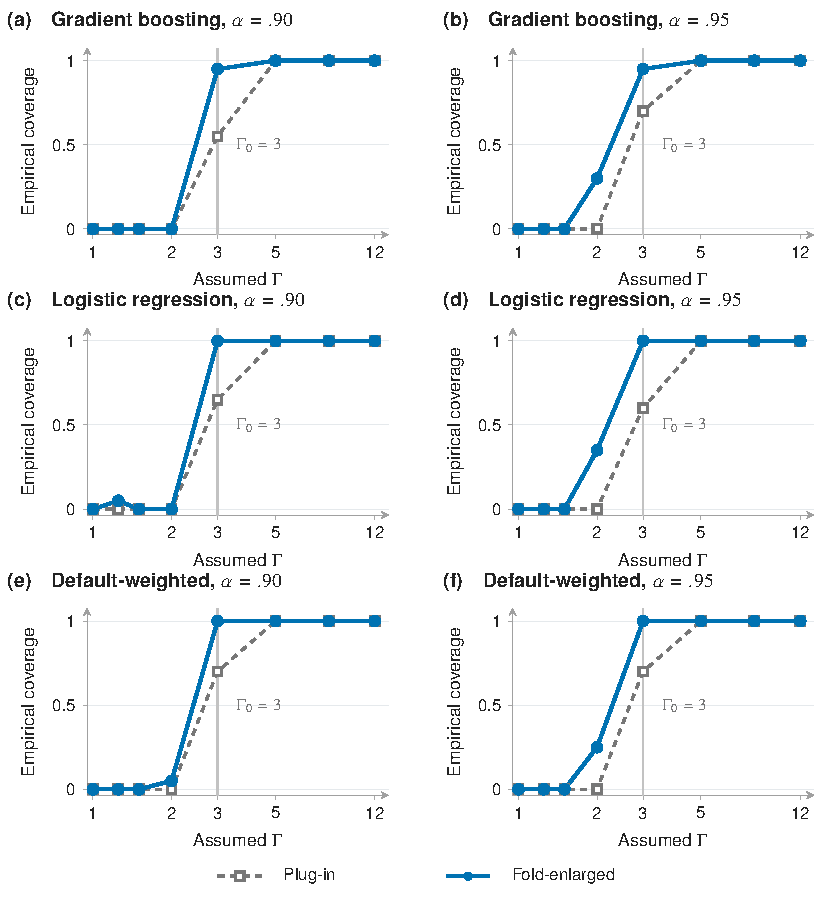
\includegraphics[width=\textwidth]{figures/supp_coverage.pdf}
\caption{\textbf{Empirical coverage by predictor and tail level.}
Each proportion uses 20 controlled masks. Blue circles show fold-enlarged intervals
and hollow gray squares plug-in intervals; the vertical reference marks the masking mechanism's sensitivity
$\Gamma_0=3$. Predictors share the same 20 masks, so the predictor-specific proportions are dependent. Default-weighted denotes default-weighted
logistic regression.}
\label{fig:detailed-coverage}
\end{figure}

\begin{samepage}
\subsection{Synthetic fixed-threshold cost--precision frontier}
\label{app:frontier-experiments}

\paragraph{Generator.}
Use 120 worlds of 120 cells, $\alpha=.85$, $\Gamma=12$, absolute loss,
$f=p_1$, and $\eta=.5$. Masses are Dirichlet$(.75,\ldots,.75)$.
Independently draw $z_j,e_j,e_j^{\rm out},e_j^{\rm in}\sim N(0,1)$ across
cells/noise types. Hidden-tail cells satisfy $z_j+.35e_j$ at or above its
empirical $.65$ quantile (NumPy default linear interpolation). Outside/inside
these cells, respectively, set
\[
p_{1j}=\operatorname{sigmoid}(-1.35+.75z_j+.45e_j^{\rm out}),\qquad
p_{1j}=\operatorname{sigmoid}(-2.05+.35z_j+.30e_j^{\rm in}),
\]
clipped to $[.04,.72]$, and draw $\pi_j\sim U[.62,.95]$/$U[.02,.16]$.
Add to the log-odds of $p_{1j}$ a shift $N(0,.18^2)$/$U[.8\log10,\log10]$
to obtain $p_{0j}$, clipped to $[.02,.98]$. Costs are $c_j=U_j+B_jV_j$ with
$U_j\sim U[.45,1.75]$, $B_j\sim\operatorname{Bernoulli}(.20)$, and
$V_j\sim U[.75,1.75]$. Primitive draws are mutually independent and independent
of masses; hidden-cell membership induces the specified dependence of $\pi_j$
and log-odds shifts on the normal scores.

The generated $p_{0j}$ specifies the hidden-outcome distribution in cell $j$. The
fixed-threshold frontier follows from
$W_{f,\eta}(\lambda)=\sum_j\mu_j(1-\lambda_j)\tau_{f,\eta}(j)$ and cost
$\sum_j\mu_jc_j\lambda_j$. The frontier calculation uses $p_1,\pi,f,\eta,\Gamma,\mu,c$; the
generated $p_0$ does not enter these formulas.
\end{samepage}

\paragraph{Allocations and equivalent baselines.}
Here $c_j$ is population cost density: allocations cost
$\sum_j\mu_jc_j\lambda_j$, with full cost $\sum_j\mu_jc_j$.
Appendix~\ref{app:finite-cell}'s fractional-knapsack solution uses useful
zero-cost cells first, then decreasing $\tau_j/c_j$ on positive-cost/value
cells (this generator has positive costs). A fractional final cell implements
51 budgets from zero to full cost in $.02$ increments. TIV/cost and the exact
frontier share this ordering and all saved coordinates.

Seven baselines rank by raw independent $U[0,1]$ random score, cell mass,
negative revelation probability, selected-label expected absolute loss,
$p_1(1-p_1)$, sensitivity width, or absolute tail-excess contrast $|d_{f,\eta}|$. Only TIV/frontier
divide their scores by cost. Each world's random scores are independent of
generator draws and reused across budgets. Decreasing NumPy default sorting
($\texttt{argsort(score)[::-1]}$) imposes no stable secondary tie rule,
including clipping-induced ties. For $v_j=p_{1j}(1-p_{1j})$, predicted loss is
$2v_j$, predictive uncertainty is $v_j$, and
\begin{equation}\label{eq:d:equivalent-baselines}
s_\Gamma(p_{1j})
=\frac{(\Gamma^2-1)v_j}{\Gamma+(\Gamma-1)^2v_j}.
\end{equation}
The last expression increases strictly in $v_j$ for $\Gamma>1$, so these three
baselines share a mathematical weak ordering and their saved curves coincide.

Normalize remaining ambiguity by its initial value within each world before
taking medians/IQR. Cost-to-target is the first recorded budget reaching 25\%
of initial ambiguity, divided by TIV's corresponding cost in that world;
there is no interpolation between budgets. Normalization requires positive
initial ambiguity, full cost, and TIV target cost. This measures divisible
population revelation at fixed $f,\eta,\Gamma$ (Theorem~\ref{thm:cert-frontier}).

\begin{figure}[!tbp]
\centering
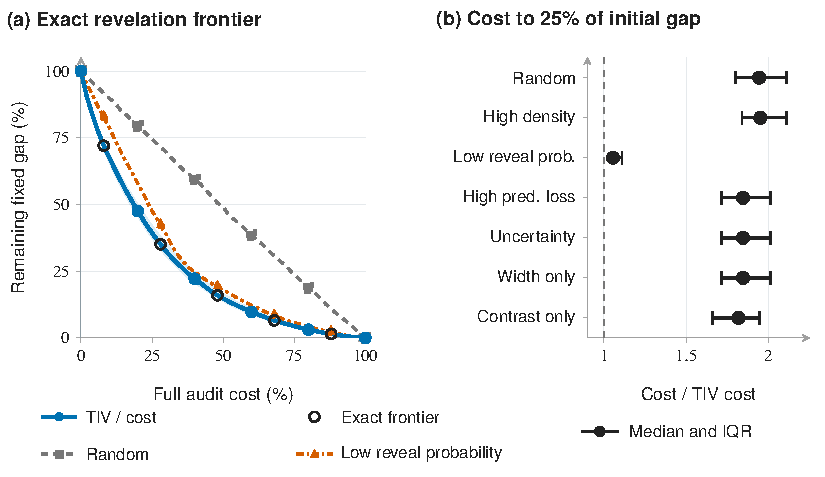
\includegraphics[width=\textwidth]{figures/supp_frontier.pdf}
\caption{\textbf{The exact revelation frontier and the cost of alternative policies.}
Across 120 finite-cell worlds, (a) median remaining fixed-threshold ambiguity,
normalized within each world; blue shading is the TIV interquartile range and
open markers identify the coincident exact frontier. (b) All seven baselines:
median cost of reaching 25\% of the initial gap relative to TIV in the same world,
with interquartile bars. Costs use the recorded 2\%-spaced grid.}
\label{fig:synthetic-frontier}
\end{figure}

\FloatBarrier
\subsection{Fixed and sequential audits of known repayments}
\label{app:repayment-audits}

Both protocols use boosting, $\alpha=.95$, $\Gamma=3$, the 20 controlled masks, and unit
cost per audited label. Let $N_{\mathrm{hidden,initial}}^{\mathrm{fix}}$ count initially
hidden cases in the fixed protocol's original pool, and let
$N_{\mathrm{hidden,initial}}^{\mathrm{seq}}$ count initially hidden cases in the sequential
protocol's 80\% training pool. Each protocol acquires eight batches of $\lceil
.02N_{\mathrm{hidden,initial}}^{\mathrm{protocol}}\rceil$ labels, capped by the remaining
eligible pool. Its budget fraction is the cumulative acquired count divided by that same
initial hidden count. Among candidates already known to be hidden, operational TIV is
$\widehat\tau/(1-\widehat\pi)=\widehat s_\Gamma|d_{f,\eta}|/\beta$, corresponding to
$c=1-\pi$ in Appendix~\ref{app:finite-cell}.

\begin{center}
\small\setlength{\tabcolsep}{3pt}
\begin{tabularx}{\textwidth}{@{}>{\raggedright\arraybackslash}p{.18\textwidth}>{\raggedright\arraybackslash}X>{\raggedright\arraybackslash}X@{}}
\toprule
Protocol & Fixed objective & Sequential retraining\\
\midrule
Data and predictor & Original hidden pool; initial cross-fitted predictor and historical nuisance predictions held fixed; upper threshold minimizes the empirical upper-endpoint objective in \eqref{eq:crossfit-endpoint}, built from the score \eqref{eq:robust-score}, before auditing. & 80/20 split jointly stratified by $(S,Y)$; acquire only in training pool, refit predictor on all known training labels each round\\
Evaluation & Empirical mean of remaining-hidden indicators times original per-label TIV; normalize by round zero within each mask & Training-pool retained plug-in width; held-out mean Brier and CVaR on the same reserved 20\%\\
Ordering/ties & One stable decreasing-score ordering per policy; ties retain masked-data order & Partial partition (\texttt{argpartition}); no stable secondary batch-cutoff rule; random scores refreshed each round\\
\bottomrule
\end{tabularx}
\end{center}

\begin{samepage}
The fixed protocol takes its upper threshold from the empirical upper-endpoint objective in
\eqref{eq:crossfit-endpoint}, built from the score \eqref{eq:robust-score}, using the
initial masking predictions of Appendix~\ref{app:controlled-masking} and the breakpoint/tie
rule of Appendix~\ref{app:historical-lending}. It freezes those predictor and nuisance
predictions, as well as this threshold, for every acquisition and fixed-gap calculation.
\par\end{samepage}

\begin{samepage}
\paragraph{Retained objective.}
Historical $p_1$ is fitted on initially revealed training outcomes, clipped as in
Appendix~\ref{app:historical-lending}, and frozen. For training size $n$, let
$A_{it}\leq1-S_i$ indicate audit by round $t$, $f_t$ be the refitted predictor,
and $\widehat p_i$ the frozen fit. The retained plug-in objective is
\begin{equation}\label{eq:d:sequential-objective}
\begin{aligned}
\widehat Q_t^\sigma(\eta)
={}&\eta+\frac{1}{n\beta}\sum_{i=1}^n\Bigl[
 S_i a^{Y_i}_{f_t,\eta}(X_i)
 +A_{it}a^{Y_i}_{f_t,\eta}(X_i)\\
&\quad +(1-S_i-A_{it})b^\sigma_{f_t,\eta}(X_i;\widehat p_i)
\Bigr],\qquad \sigma\in\{L,U\}.
\end{aligned}
\end{equation}
\end{samepage}
Known outcomes enter directly; still-hidden outcomes retain historical
sensitivity envelopes. Each endpoint uses breakpoint minimization, the threshold
tie rule, clipping, and midpoint collapse of Appendix~\ref{app:historical-lending}.
At full revelation $A_{it}=1-S_i$, both objectives equal
$\eta+(n\beta)^{-1}\sum_i a^{Y_i}_{f_t,\eta}(X_i)$ and both endpoints equal
full-training-data empirical CVaR; a regression test verifies this identity.
These training-prediction widths and held-out predictive risks are descriptive
trajectories, without fold enlargement or adaptive confidence guarantees.

\paragraph{Acquisition rules.}
Among still-hidden candidates, let $\widehat p_{\mathrm{known}}$ denote the fitted outcome
probability from currently known labels, and let $\widehat s_\Gamma=q_+(\widehat
p_1)-q_-(\widehat p_1)$ be the sensitivity width from the frozen historical outcome fit. In
the sequential protocol, let $\widehat\eta^U$ be the current upper-endpoint minimizing
threshold of \eqref{eq:d:sequential-objective}. The six acquisition scores are TIV per label
cost $\widehat s_\Gamma|d_{f,\widehat\eta^U}|/(\beta\kappa)$, with $\kappa=1$; independent
uniform random scores; predictive uncertainty $1-2|f-.5|$; negative fitted probability of
currently having a known label; predicted Brier loss $(1-\widehat
p_{\mathrm{known}})f^2+\widehat p_{\mathrm{known}}(1-f)^2$; and historical sensitivity width
$\widehat s_\Gamma$. The fixed protocol uses its frozen initial predictor, threshold, and
historical fits. Sequential TIV uses the current predictor and upper threshold with the
frozen historical sensitivity bounds. The propensity baseline refits the indicator of a
currently known label on all training covariates, with probabilities clipped to $[.02,.98]$.
Predicted loss refits the outcome model on currently known outcomes and uses its raw
probabilities. These models share the boosting settings above, with their respective
targets, available labels, and seeds. Refreshed acquisition fits guide label choice;
retained evaluation continues to use the historical outcome fit in
\eqref{eq:d:sequential-objective}.

\begin{table}[!htbp]
\centering\small
\begin{tabular}{@{}lrr@{}}
\toprule
Acquisition rule & \shortstack[r]{Fixed-threshold\\gap reduction}
& \shortstack[r]{Final median sequential\\interval width}\\
\midrule
TIV per label cost & 61\% & .035\\
Random & 16\% & .067\\
Lowest revelation propensity & 9\% & .084\\
Predicted loss & 0\% & .116\\
Predictive uncertainty & 0\% & .116\\
Sensitivity width & 0\% & .116\\
\bottomrule
\end{tabular}
\caption{Complete fixed and sequential audit comparison at the nominal 16\%
budget. Fixed reductions are medians of within-mask percentage reductions;
estimated sequential widths are medians across the 20 runs. Integer rounding gives actual median budget fractions of 16.013\% of the fixed initial hidden pool and 16.018\% of the sequential initial hidden training pool.}
\label{tab:audit-protocols}
\end{table}

\begin{table}[!htbp]
\centering\small
\begin{tabular}{lccc}
\toprule
Acquisition rule & Estimated width & Mean Brier & CVaR\\
\midrule
TIV & 0.0348 & 0.1362 & 0.8541\\
Random & 0.0671 & 0.1347 & 0.8682\\
Paired TIV$-$Random & $-0.0332$ & $+0.0014$ & $-0.0138$\\
\midrule
\multicolumn{4}{l}{\textit{Exact predictor reference}}\\
Constant $f\equiv1/2$ & 0.0000 & 0.2500 & 0.2500\\
\bottomrule
\end{tabular}
\par\smallskip{\footnotesize The constant forecast supplies an exact predictor reference.}

\caption{Precision and predictive loss after eight equal-budget audit rounds.
Policy rows are medians across 20 masks; the paired row is the median of the
within-mask TIV-minus-random differences. Estimated width uses the training pool;
mean Brier loss and CVaR use the same reserved 20\% split.}
\label{tab:sequential-performance}
\end{table}

\FloatBarrier
\begin{samepage}
In all 20 paired terminal runs, TIV has lower estimated width and held-out CVaR than random,
while random has lower mean Brier loss. The median paired differences are $-.0332$ in width,
$-.0138$ in CVaR, and $+.0014$ in mean Brier loss (Table~\ref{tab:sequential-performance}). The
exact constant reference has lower tail loss and higher mean loss than both policy medians.
Figure~\ref{fig:all-revelation} shows how the estimated width and held-out tail risk evolve
as each policy changes the training labels and predictor.

\par\end{samepage}

\begin{figure}[!htbp]
\centering
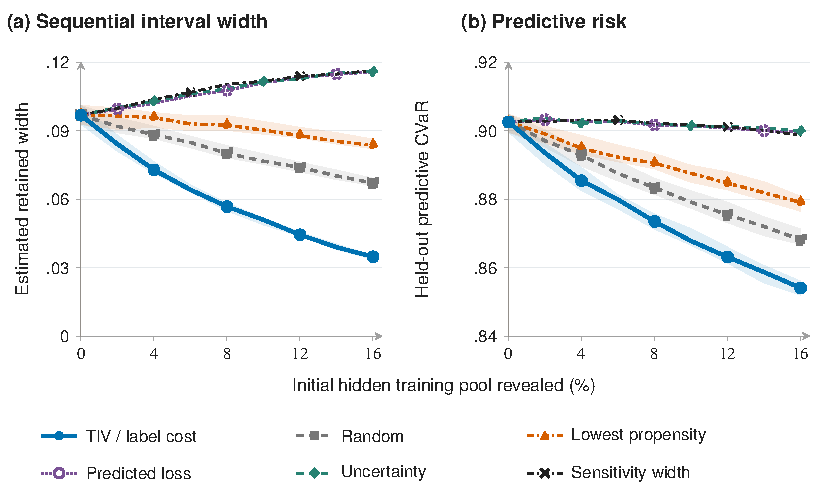
\includegraphics[width=\textwidth]{figures/supp_revelation.pdf}
\caption{\textbf{Sequential precision and predictive outcomes across all six acquisition rules.}
Lines are medians over 20 masks at $\alpha=.95$, $\Gamma=3$; light bands are interquartile
ranges for TIV, random, and lowest-propensity acquisition. (a) Estimated
retained-sensitivity width for the current predictor. (b) Its CVaR on the reserved 20\%
split. Predicted-loss, predictive-uncertainty, and sensitivity-width curves are plotted
separately and nearly overlap. Lines join recorded rounds.
Table~\ref{tab:sequential-performance} gives the exact constant-forecast reference. The horizontal coordinate is the median fraction of initially hidden training-pool labels acquired.}
\label{fig:all-revelation}
\end{figure}

\FloatBarrier
\begin{samepage}
\subsection{Recorded implementation inventory}
\label{app:implementation-inventory}

The accompanying \path{reproducibility/README.md} and
\path{reproducibility/implementation_inventory.tex} record implementation entry points,
configurations, seeds, draw order, saved-output mappings, and runtime/hash logs. The
sequential results in Figure~\ref{fig:revelation-results}b, Figure~\ref{fig:all-revelation},
and Tables~\ref{tab:audit-protocols}--\ref{tab:sequential-performance} use the retained
plug-in objective \eqref{eq:d:sequential-objective}; the inventory identifies its runner and
configuration and records residual-corrected trajectories separately. It also documents the
cohort verification: all 53,367 reconstructed issued records match all 12 shared columns in
their original order, and all 20 archived mask diagnostics match.

\par\end{samepage}

\FloatBarrier
